\documentclass[11pt, a4paper]{article}

% --- Packages ----------------------------------------------------------------
\usepackage[utf8]{inputenc}
\usepackage[T1]{fontenc}
\usepackage[margin=2.5cm]{geometry}
\usepackage{graphicx}
\usepackage{hyperref}
\usepackage{booktabs}       % nicer tables (\toprule, \midrule, \bottomrule)
\usepackage{float}          % [H] placement for figures and tables
\usepackage{xcolor}         % colors (used by listings)
\usepackage{listings}       % code listings
\hypersetup{colorlinks=true, linkcolor=black, citecolor=black, urlcolor=blue!70!black}

% --- Code listing style -----------------------------------------------------
\lstset{
    basicstyle=\ttfamily\small,
    breaklines=true,
    frame=single,
    numbers=left,
    numberstyle=\tiny\color{gray},
    xleftmargin=2em,
    framexleftmargin=1.5em
}
% Pro tip: for syntax highlighting, look into the 'minted' package.

% --- Bibliography ------------------------------------------------------------
\usepackage[style=numeric, backend=bibtex]{biblatex}
\addbibresource{references.bib}

% --- Language (swap to lang/sk for Slovak) -----------------------------------
\input{lang/en}

% --- Student details ---------------------------------------------------------
\newcommand{\StudentName}{Bohdan Karpenko, Arseniy Malyuk, Oleksii Khmelevskyi}
\newcommand{\StudyGroup}{Wednesday 14:00}
\newcommand{\AssignmentNumber}{3}
\newcommand{\AssignmentTitle}{Cinema}
\newcommand{\AcademicYear}{2025/2026}

% =============================================================================
\begin{document}

% --- Cover page --------------------------------------------------------------
\begin{titlepage}
    \centering

    \includegraphics[width=0.3\textwidth]{../assets/logo}

    \vspace{0.3cm}
    {\large \LabelUniversity}\\[2pt]
    {\large \LabelFaculty}

    \vspace{2.5cm}
    {\Huge\bfseries \LabelProtocol}

    \vspace{0.6cm}
    {\LARGE \LabelCode{} --- \LabelCourse}

    \vspace{0.4cm}
    {\Large \LabelAssignment{} \AssignmentNumber: \AssignmentTitle}

    \vfill

    \begin{tabular}{r l}
        \textbf{\LabelStudent:} & \StudentName  \\[4pt]
        \textbf{\LabelGroup:}   & \StudyGroup   \\[4pt]
        \textbf{\LabelYear:}    & \AcademicYear \\[4pt]
        \textbf{\LabelDate:}    & \today        \\
    \end{tabular}

    \vspace{1.5cm}
\end{titlepage}

% --- Table of contents -------------------------------------------------------
\renewcommand{\contentsname}{\LabelContents}
\tableofcontents
\newpage


\section{Physical Model – Implementation}

\subsection{List of Tables}
The following tables have been implemented to represent the cinema management system:

\begin{itemize}
    \item \textbf{staffs}: Stores employee information, including names, age, and professional positions.
    \item \textbf{halls}: Contains data regarding cinema auditoriums, their names, and seating capacities.
    \item \textbf{films}: A catalog of movies featuring titles, durations, and age ratings.
    \item \textbf{actors}: A registry of actors (first and last names) performing in the films.
    \item \textbf{genres}: A lookup table for various movie genres available in the system.
    \item \textbf{studios}: A registry of production studios responsible for the films.
    \item \textbf{screenings}: Scheduled movie showtimes, linking films to specific halls and times.
    \item \textbf{shifts}: Employee work schedules, including descriptions and time intervals.
    \item \textbf{sales}: Records of ticket transactions, linking customers to specific screenings.
    \item \textbf{actors\_films}: Junction table managing the M:N relationship between actors and films.
    \item \textbf{films\_genres}: Junction table for assigning multiple genres to films (M:N).
    \item \textbf{films\_studios}: Junction table linking films to their respective production studios.
    \item \textbf{shifts\_screenings}: Junction table assigning staff shifts to the screenings they service.
\end{itemize}

\subsection{Notable Integrity Constraints}
The following constraints were implemented to enforce specific business rules and ensure data validity:

\begin{itemize}
    \item \textbf{Employee Age (CHECK)}: The constraint \texttt{age >= 15} in the \texttt{staffs} table ensures that the cinema complies with labor regulations allowing the employment of teenagers from the age of 15.
    \item \textbf{Auditorium Capacity (CHECK)}: The \texttt{capacity > 0} condition in the \texttt{halls} table prevents the creation of invalid rooms with no seating.
    \item \textbf{Film Duration (CHECK)}: The \texttt{duration} field must be a positive integer, eliminating data entry errors for movie lengths.
    \item \textbf{Genre Uniqueness (UNIQUE)}: Ensures that genre names are not duplicated, maintaining a clean and consistent categorization system.
    \item \textbf{Referential Integrity}: All foreign keys ensure that child records (e.g., sales, screenings) always point to existing parent records, preventing orphaned data.
\end{itemize}

\subsection{Selected Referential Actions}
To maintain database consistency and prevent accidental data loss, the following strategies were applied to all foreign key relationships:

\begin{itemize}
    \item \textbf{ON DELETE RESTRICT}: This strategy is used across all tables to prevent the deletion of a parent record if any referenced child records exist. For example, a film cannot be deleted if there are existing screenings or sales associated with it. This ensures the preservation of historical data and prevents "orphaned" records that would break the system's logic.
    \item \textbf{ON UPDATE CASCADE}: This strategy ensures that any changes to primary keys (e.g., updating a unique identifier) are automatically propagated to all related foreign keys in child tables. This maintains seamless connectivity between entities without manual intervention after an update.
\end{itemize}
\newpage


\section{Seed Data}

\subsection{Data Generation Process}
The dataset was programmatically generated using a custom \textbf{Python} script and the \textbf{Faker} library. A fixed seed (\texttt{Faker.seed(67)}) was used to ensure reproducibility. The script handles complex logic such as:
\begin{itemize}
    \item String truncation to fit \texttt{VARCHAR(32)} constraints.
    \item Ensuring uniqueness for studio and genre names.
    \item Maintaining referential integrity by generating data in a specific hierarchical order.
\end{itemize}

\subsection{Record Counts}
After executing the \texttt{seed.sql} script, the database contains over 14,000 records. The precise distribution is summarized in the table below:

\begin{table}[h!]
\centering
\begin{tabular}{lr}
\toprule
\textbf{Table Name} & \textbf{Record Count} \\
\midrule
staffs & 30 \\
halls & 8 \\
films & 200 \\
actors & 200 \\
genres & 15 \\
studios & 20 \\
screenings & 1,000 \\
sales & 10,000 \\
shifts & 300 \\
\midrule
\textit{Junction Tables:} & \\
actors\_films & 596 \\
films\_genres & 318 \\
films\_studios & 311 \\
shifts\_screenings & 1,365 \\
\midrule
\textbf{Total Records} & \textbf{14,363} \\
\bottomrule
\end{tabular}
\caption{Final record counts after database seeding.}
\end{table}

\subsection{Data Distribution and Consistency}
The distribution of data reflects a realistic cinema operations model:
\begin{itemize}
    \item \textbf{High-Volume Sales}: 10,000 sales across 1,000 screenings simulate a realistic average of 10 tickets sold per screening.
    \item \textbf{Junction Table Logic}: 
    \begin{itemize}
        \item \textbf{Actors/Films}: On average, 3 actors are assigned per film (596 records for 200 films).
        \item \textbf{Shifts/Screenings}: Each staff shift (300 total) covers approximately 4.5 screenings, representing a standard 8-hour workday.
    \end{itemize}
    \item \textbf{Temporal Integrity}: All screenings and shifts are generated within a one-year window, ensuring that the scheduling system remains logically consistent for analytical queries.
\end{itemize}
\newpage


\section{Design of the Relational Model}
\label{sec:implementation}

\subsection{Relational Model Diagram}

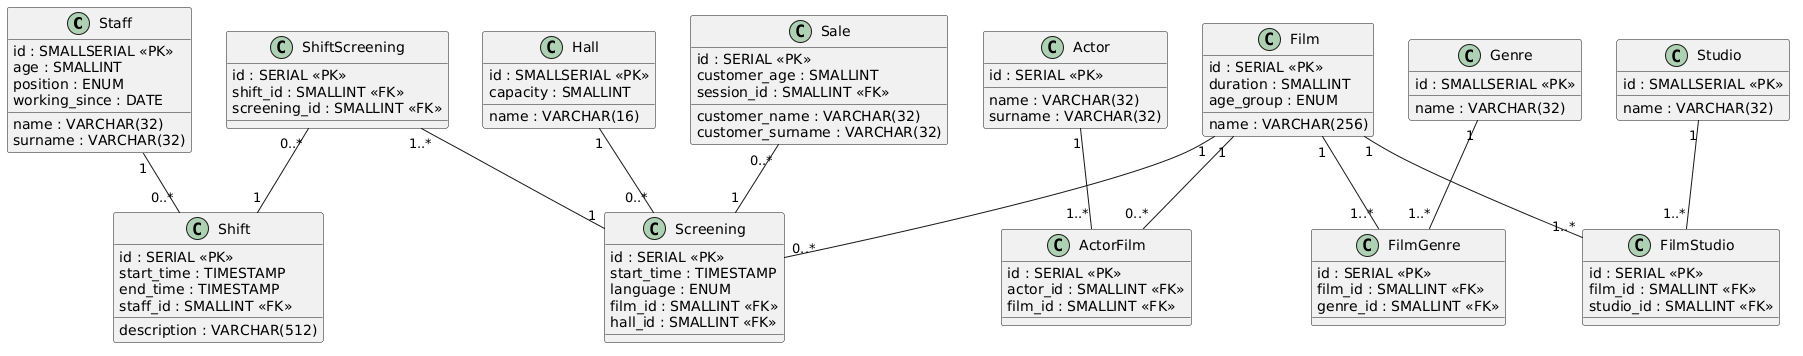
\includegraphics[width=1\textwidth]{../assets/UML}

\subsection{Table Descriptions}

All primary keys are surrogate keys of type \texttt{SMALLSERIAL}. This approach provides better performance for joins and ensures that the primary identifier remains immutable even if business data (such as a film title or employee name) changes.

\bigskip

% 1. STAFF
\textbf{Table: Staff} \\
\textit{Purpose:} Stores information about employees.
\begin{itemize}
    \item \textbf{Attributes:}
    \begin{itemize}
        \item \texttt{id} (\texttt{SMALLSERIAL}): PK, NOT NULL. Unique identifier.
        \item \texttt{name} (\texttt{VARCHAR(32)}): NOT NULL.
        \item \texttt{surname} (\texttt{VARCHAR(32)}): NOT NULL.
        \item \texttt{age} (\texttt{SMALLINT}): CHECK (age $\ge$ 15).
        \item \texttt{position} (\texttt{ENUM}): NOT NULL. Role within the cinema.
        \item \texttt{working\_since} (\texttt{DATE}): DEFAULT CURRENT\_DATE.
    \end{itemize}
    \item \textbf{PK Choice:} Artificial (\texttt{id}). Natural keys (name + surname) are non-unique.
\end{itemize}

% 2. SHIFT
\textbf{Table: Shift} \\
\textit{Purpose:} Logs the working hours assigned to specific staff members.
\begin{itemize}
    \item \textbf{Attributes:}
    \begin{itemize}
        \item \texttt{id} (\texttt{SMALLSERIAL}): PK, NOT NULL. Unique identifier.
        \item \texttt{description} (\texttt{VARCHAR(512)}): Description of work for shift.
        \item \texttt{start\_time} (\texttt{TIMESTAMP}): NOT NULL.
        \item \texttt{end\_time} (\texttt{TIMESTAMP}): NOT NULL, CHECK (end\_time $>$ start\_time).
        \item \texttt{staff\_id} (\texttt{SMALLINT}): FK, NOT NULL. References \texttt{Staff(id)}.
    \end{itemize}
    \item \textbf{PK Choice:} Artificial (\texttt{id}).
\end{itemize}

% 3. SHIFTSCREENING
\textbf{Table: ShiftScreening} \\
\textit{Purpose:} Junction table realizing the M:N relationship between Shifts and Screenings.
\begin{itemize}
    \item \textbf{Attributes:}
    \begin{itemize}
        \item \texttt{id} (\texttt{SMALLSERIAL}): PK, NOT NULL. Unique identifier.
        \item \texttt{shift\_id} (\texttt{SMALLINT}): FK, NOT NULL. References \texttt{Shift(id)}.
        \item \texttt{screening\_id} (\texttt{SMALLINT}): FK, NOT NULL. References \texttt{Screening(id)}.
    \end{itemize}
\end{itemize}

% 4. SCREENING
\textbf{Table: Screening} \\
\textit{Purpose:} Represents a specific instance of a film being shown in a hall.
\begin{itemize}
    \item \textbf{Attributes:}
    \begin{itemize}
        \item \texttt{id} (\texttt{SMALLSERIAL}): PK, NOT NULL. Unique identifier.
        \item \texttt{start\_time} (\texttt{TIMESTAMP}): NOT NULL.
        \item \texttt{language} (\texttt{ENUM}): Audio/Subtitle configuration.
        \item \texttt{film\_id} (\texttt{SMALLINT}): FK, NOT NULL. References \texttt{Film(id)}.
        \item \texttt{hall\_id} (\texttt{SMALLINT}): FK, NOT NULL. References \texttt{Hall(id)}.
    \end{itemize}
    \item \textbf{PK Choice:} Artificial (\texttt{id}).
\end{itemize}

% 5. HALL
\textbf{Table: Hall} \\
\textit{Purpose:} Defines the physical spaces where screenings occur.
\begin{itemize}
    \item \textbf{Attributes:}
    \begin{itemize}
        \item \texttt{id} (\texttt{SMALLSERIAL}): PK, NOT NULL. Unique identifier.
        \item \texttt{name} (\texttt{VARCHAR(16)}): UNIQUE, NOT NULL.
        \item \texttt{capacity} (\texttt{SMALLINT}): NOT NULL, CHECK (capacity $>$ 0).
    \end{itemize}
    \item \textbf{PK Choice:} Artificial (\texttt{id}). Allows for renaming halls without breaking relations.
\end{itemize}

% 6. SALE
\textbf{Table: Sale} \\
\textit{Purpose:} Records ticket transactions and customer data.
\begin{itemize}
    \item \textbf{Attributes:}
    \begin{itemize}
        \item \texttt{id} (\texttt{SMALLSERIAL}): PK, NOT NULL. Unique identifier.
        \item \texttt{customer\_name} (\texttt{VARCHAR(32)}): NOT NULL.
        \item \texttt{customer\_surname} (\texttt{VARCHAR(32)}): NOT NULL.
        \item \texttt{customer\_age} (\texttt{SMALLINT}): CHECK (customer\_age $\ge$ 0).
        \item \texttt{screening\_id} (\texttt{SMALLINT}): FK, NOT NULL. References \texttt{Screening(id)}.
    \end{itemize}
    \item \textbf{PK Choice:} Artificial (\texttt{id}).
\end{itemize}

% 7. FILM
\textbf{Table: Film} \\
\textit{Purpose:} Stores information about films that have been, are, and will be shown in the cinema.
\begin{itemize}
    \item \textbf{Attributes:}
    \begin{itemize}
        \item \texttt{id} (\texttt{SMALLSERIAL}): PK, NOT NULL. Unique identifier.
        \item \texttt{name} (\texttt{VARCHAR(256)}): NOT NULL.
        \item \texttt{duration} (\texttt{SMALLINT}): NOT NULL, CHECK (duration $>$ 0).
        \item \texttt{age\_group} (\texttt{ENUM}): Rating for content suitability.
    \end{itemize}
    \item \textbf{PK Choice:} Artificial (\texttt{id}). Film titles can be remade or duplicated.
\end{itemize}

% 8. ACTORFILM
\textbf{Table: ActorFilm} \\
\textit{Purpose:} Junction table realizing the M:N relationship between Actors and Films.
\begin{itemize}
    \item \textbf{Attributes:}
    \begin{itemize}
        \item \texttt{id} (\texttt{SMALLSERIAL}): PK, NOT NULL. Unique identifier.
        \item \texttt{actor\_id} (\texttt{SMALLINT}): FK, NOT NULL. References \texttt{Actor(id)}.
        \item \texttt{film\_id} (\texttt{SMALLINT}): FK, NOT NULL. References \texttt{Film(id)}.
    \end{itemize}
\end{itemize}

% 9. ACTOR
\textbf{Table: Actor} \\
\textit{Purpose:} Stores information about actors participating in films.
\begin{itemize}
    \item \textbf{Attributes:}
    \begin{itemize}
        \item \texttt{id} (\texttt{SMALLSERIAL}): PK, NOT NULL. Unique identifier.
        \item \texttt{name} (\texttt{VARCHAR(32)}): NOT NULL.
        \item \texttt{surname} (\texttt{VARCHAR(32)}): NOT NULL.
    \end{itemize}
    \item \textbf{PK Choice:} Artificial (\texttt{id}). Natural keys (name + surname) are non-unique.
\end{itemize}

% 10. FILMGENRE
\textbf{Table: FilmGenre} \\
\textit{Purpose:} Junction table realizing the M:N relationship between Films and Genres.
\begin{itemize}
    \item \textbf{Attributes:}
    \begin{itemize}
        \item \texttt{id} (\texttt{SMALLSERIAL}): PK, NOT NULL.
        \item \texttt{film\_id} (\texttt{SMALLINT}): FK, NOT NULL. References \texttt{Film(id)}.
        \item \texttt{genre\_id} (\texttt{SMALLINT}): FK, NOT NULL. References \texttt{Genre(id)}.
    \end{itemize}
\end{itemize}

% 11. GENRE
\textbf{Table: Genre} \\
\textit{Purpose:} A dictionary table for film genre categories.
\begin{itemize}
    \item \textbf{Attributes:}
    \begin{itemize}
        \item \texttt{id} (\texttt{SMALLSERIAL}): PK, NOT NULL.
        \item \texttt{name} (\texttt{VARCHAR(32)}): UNIQUE, NOT NULL.
    \end{itemize}
    \item \textbf{PK Choice:} Artificial (\texttt{id}).
\end{itemize}

% 12. FILMSTUDIO
\textbf{Table: FilmStudio} \\
\textit{Purpose:} Junction table realizing the M:N relationship between Films and Studios.
\begin{itemize}
    \item \textbf{Attributes:}
    \begin{itemize}
        \item \texttt{id} (\texttt{SMALLSERIAL}): PK, NOT NULL.
        \item \texttt{film\_id} (\texttt{SMALLINT}): FK, NOT NULL. References \texttt{Film(id)}.
        \item \texttt{studio\_id} (\texttt{SMALLINT}): FK, NOT NULL. References \texttt{Studio(id)}.
    \end{itemize}
\end{itemize}

% 13. STUDIO
\textbf{Table: Studio} \\
\textit{Purpose:} Stores information about film production studios.
\begin{itemize}
    \item \textbf{Attributes:}
    \begin{itemize}
        \item \texttt{id} (\texttt{SMALLSERIAL}): PK, NOT NULL.
        \item \texttt{name} (\texttt{VARCHAR(32)}): UNIQUE, NOT NULL.
    \end{itemize}
    \item \textbf{PK Choice:} Artificial (\texttt{id}).
\end{itemize}
\newpage


\subsection{Description of Relationships}

\begin{table}[h]
\centering
\small
\begin{tabular}{|l|c|l|c|l|}
\hline
\textbf{Relationship} & \textbf{Type} & \textbf{Physical Realization} & \textbf{Optionality} \\ \hline
Staff $\rightarrow$ Shift & 1:N & FK in Shift & Optional \\
Shift $\rightarrow$ ShiftScreening & 1:N & FK in ShiftScreening & Optional \\
Screening $\rightarrow$ ShiftScreening & 1:N & FK in ShiftScreening & Optional \\
Hall $\rightarrow$ Screening & 1:N & FK in Screening & Optional \\
Screening $\rightarrow$ Sale & 1:N & FK in Sale & Optional \\
Film $\rightarrow$ Screening & 1:N & FK in Screening & Optional \\
Film $\rightarrow$ ActorFilm & 1:N & FK in ActorFilm & Optional \\
Actor $\rightarrow$ ActorFilm & 1:N & FK in ActorFilm & Mandatory \\
Film $\rightarrow$ FilmGenre & 1:N & FK in FilmGenre & Mandatory \\
Genre $\rightarrow$ FilmGenre & 1:N & FK in FilmGenre & Mandatory \\
Film $\rightarrow$ FilmStudio & 1:N & FK in FilmStudio & Mandatory \\
Studio $\rightarrow$ FilmStudio & 1:N & FK in FilmStudio & Mandatory \\
\hline
\end{tabular}
\end{table}

\subsubsection{Referential Integrity: ON DELETE Actions}

\begin{table}[h]
\centering
\small
\begin{tabular}{|l|l|}
\hline
\textbf{Table} & \textbf{ON DELETE Action} \\ \hline
\texttt{Staff} & \texttt{RESTRICT} \\ \hline
\texttt{Shift} & \texttt{RESTRICT} \\ \hline
\texttt{ShiftScreening} & \texttt{RESTRICT} \\ \hline
\texttt{Screening} & \texttt{RESTRICT} \\ \hline
\texttt{Hall} & \texttt{RESTRICT} \\ \hline
\texttt{Sale} & \texttt{RESTRICT} \\ \hline
\texttt{Film} & \texttt{RESTRICT} \\ \hline
\texttt{ActorFilm} & \texttt{RESTRICT} \\ \hline
\texttt{Actor} & \texttt{RESTRICT} \\ \hline
\texttt{FilmGenre} & \texttt{RESTRICT} \\ \hline
\texttt{Genre} & \texttt{RESTRICT} \\ \hline
\texttt{FilmStudio} & \texttt{RESTRICT} \\ \hline
\texttt{Studio} & \texttt{RESTRICT} \\ \hline
\end{tabular}
\end{table}

\subsection{Integrity Constraints Realization}

The integrity constraints described in Chapter 2 (Specification) are implemented in the relational model using a combination of structural constraints, domain restrictions, and business logic checks.

\begin{itemize}

\item \textbf{Film information completeness}

According to the specification, every film must contain a title, duration, studio, actors, and genres.

This requirement is implemented using:
\begin{itemize}
    \item \texttt{NOT NULL} constraints on \texttt{Film.name} and \texttt{Film.duration}.
    \item A \texttt{CHECK (duration > 0)} constraint to ensure valid film length.
    \item Junction tables \texttt{ActorFilm}, \texttt{FilmGenre}, and \texttt{FilmStudio} that associate films with actors, genres, and studios.
\end{itemize}

\item \textbf{Hall capacity limitation}

A ticket cannot be sold if the number of sold tickets exceeds the capacity of the hall where the screening is held.

This rule is implemented by:
\begin{itemize}
    \item Storing hall capacity in the \texttt{Hall.capacity} attribute.
    \item Linking ticket sales to screenings through the \texttt{Sale.screening\_id} foreign key.
    \item Verifying during ticket insertion that the number of existing sales for a screening does not exceed the capacity of the related hall. This rule can be implemented using an application-level validation.
\end{itemize}

\item \textbf{Age restriction for films}

A ticket cannot be sold if the customer's age does not satisfy the age rating of the film.

This rule is enforced by:
\begin{itemize}
    \item Storing the film rating in the \texttt{Film.age\_group} attribute.
    \item Recording the customer's age in \texttt{Sale.customer\_age}.
    \item Comparing these values during ticket purchase using an application-level validation.
\end{itemize}

\item \textbf{Non-overlapping screenings in the same hall}

At any given time only one screening can take place in a hall.

This constraint is implemented by:
\begin{itemize}
    \item Storing the start time of each screening in \texttt{Screening.start\_time}.
    \item Linking screenings to halls using the \texttt{hall\_id} foreign key.
    \item Checking that the time interval of a new screening does not overlap with existing screenings in the same hall.
\end{itemize}

\item \textbf{General relational integrity}

Basic database integrity is ensured through:
\begin{itemize}
    \item \textbf{Entity integrity}: every table has a \texttt{PRIMARY KEY} (\texttt{id}).
    \item \textbf{Referential integrity}: relationships between entities are enforced using \texttt{FOREIGN KEY} constraints.
    \item \textbf{Domain integrity}: implemented using appropriate data types and \texttt{CHECK} constraints (for example age limits, positive durations, and valid shift times).
\end{itemize}

\end{itemize}

These mechanisms ensure that the database structure enforces the main business rules defined in the system specification.
\subsection{User Scenario Verification}

The proposed relational model fully supports the required system functionality:

\begin{itemize}
    \item \textbf{Purchasing \& Information (Scenarios 1, 2, 6):} Handled by \texttt{Film}, \texttt{Screening}, and \texttt{Sale} tables. Metadata (actors, genres, studios) is managed through junction tables (\texttt{ActorFilm}, \texttt{FilmGenre}, \texttt{FilmStudio}).
    \item \textbf{Session Management (Scenarios 4):} Administrators manage the \texttt{Screening} table. The \texttt{hall\_id} and \texttt{start\_time} attributes allow for overlap checks and scheduling.
    \item \textbf{Staff \& Shifts (Scenarios 3, 5):} Personnel work hours are tracked in the \texttt{Shift} table. Responsibility for specific screenings is recorded via the \texttt{ShiftScreening} junction table, linking \texttt{Staff} to \texttt{Screening}.
\end{itemize}
% \newpage


\section{Evaluation and Conclusion}
\label{sec:evaluation}

The proposed solution implements the basic logic of a potential cinema.
The scheme does not implement budget calculation and salary payment, specific events within the cinema, does not allow creating accounts on the platform, etc.

Creating the logic model and tables took the most time because it required the most planning and thinking through all possible further requirements and problems from use.

The problems included having difficulties with understanding what logic to implement with \textbf{ON DELETE} actions,
we learned that in practice most tables use \texttt{RESTRICT}, therefore it was implemented as such.

Some of us have never worked with databases before, therefore this whole experience was quite new and learning-intensive.

The development process was built around requirements generation and adapting the database schema to meet these requirements.
That said, it was a very iterative process, and we had to go back and forth between the specification and the implementation several times to ensure that all requirements were properly addressed in the database design.

AI was used to assist with formatting the text style since \LaTeX\ is not used much by us.

This topic was chosen because of its versatility to form a fairly simple data scheme with a few tables and also deepen it by adding more details and complex dependencies.

\end{document}